\section{Evaluation\label{sec:evaluation}}
TimeTubesX is a browser-based application written in HTML and Javascript.
We use React.js to build user interfaces and flux.js to manage the application states.
We also utilize standard libraries such as three.js~\cite{three_framework}, D3.js~\cite{d3_framework}, and Paper.js~\cite{paper_framework}.
TimeTubesX is open-source (\url{https://github.com/MistletoeNaoko/TimeTubesWeb}), and 
readers can try the running system using our synthetic data at \url{https://timetubes.herokuapp.com/}.

We shared TimeTubesX with four domain experts, three of whom we interviewed for the domain analysis in Section~\ref{sec:domainGoalsandTasks}: the second author of this paper (Astronomer 1), Astronomer 1’s former master course student (Astronomer 2), an assistant professor at Hiroshima University (Astronomer 3), and a postdoctoral researcher at Stanford University (Astronomer 4). Sections \ref{sec:correlate} and \ref{sec:anticorrelate} present two case studies conducted by Astronomer 1, and Section \ref{sec:whatif} discusses the cause of the phenomena presented in Section \ref{sec:anticorrelate}. Section \ref{sec:feedback} reviews qualitative feedback from the four domain experts.
To examine the magnetic field structures in the jets, 
astronomers analyze polarimetric observations. 
Through the analysis of correlations between polarization and intensity, 
they validate multiple hypotheses for the increase in the intensity ($I$). 
In the two case studies, Astronomer 1 used the datasets for the blazar \emph{BL Lac}.
It was empirically noted in \cite{Gaur2014} that the $I$ of \emph{BL Lac} tends to anticorrelate with the polarization degree ($PD$) during a certain period.
On a MacBook Pro 2017 with a 3.5 GHz Intel Core i7 and a 16 GB RAM, it took 1{,}193 ms and 1{,}236 ms to obtain the results outlined in Sections~\ref{sec:correlate} and \ref{sec:anticorrelate}, respectively.

\subsection{Case Study 1: Correlation Patterns of $I$ and $PD$}\label{sec:correlate}
\begin{figure}[tb]
    \centering
    \begin{minipage}{0.49\linewidth}
        \centering
        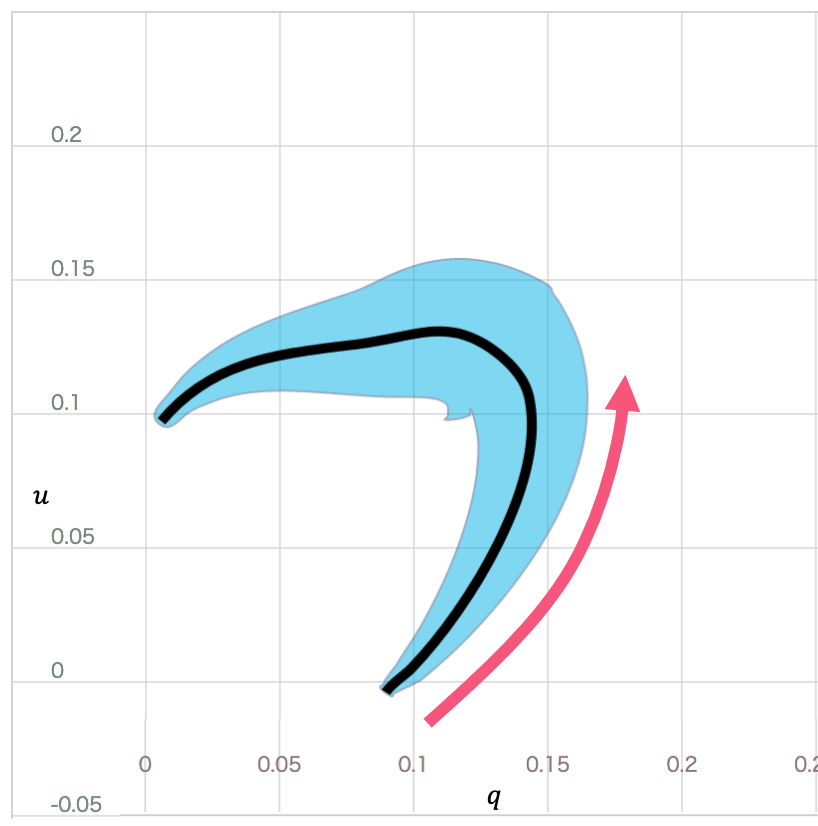
\includegraphics[width=.9\linewidth]{figures/QBScorrelate.png}\\
        \footnotesize{\sf(a)~A query for a correlated $I$ and $PD$ variation.}\\
    \end{minipage}
    \begin{minipage}{0.49\linewidth}
        \centering
        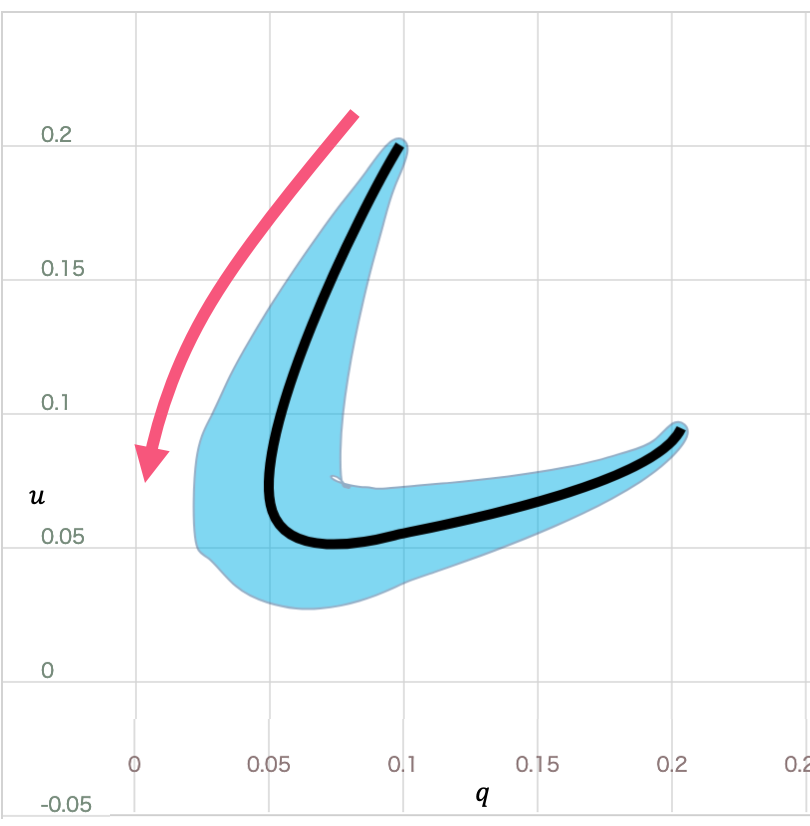
\includegraphics[width=.9\linewidth]{figures/QBSanticorrelate.png}\\
        \footnotesize{\sf(b)~A query for an anticorrelated $I$ and $PD$ variation.}\\
    \end{minipage}
    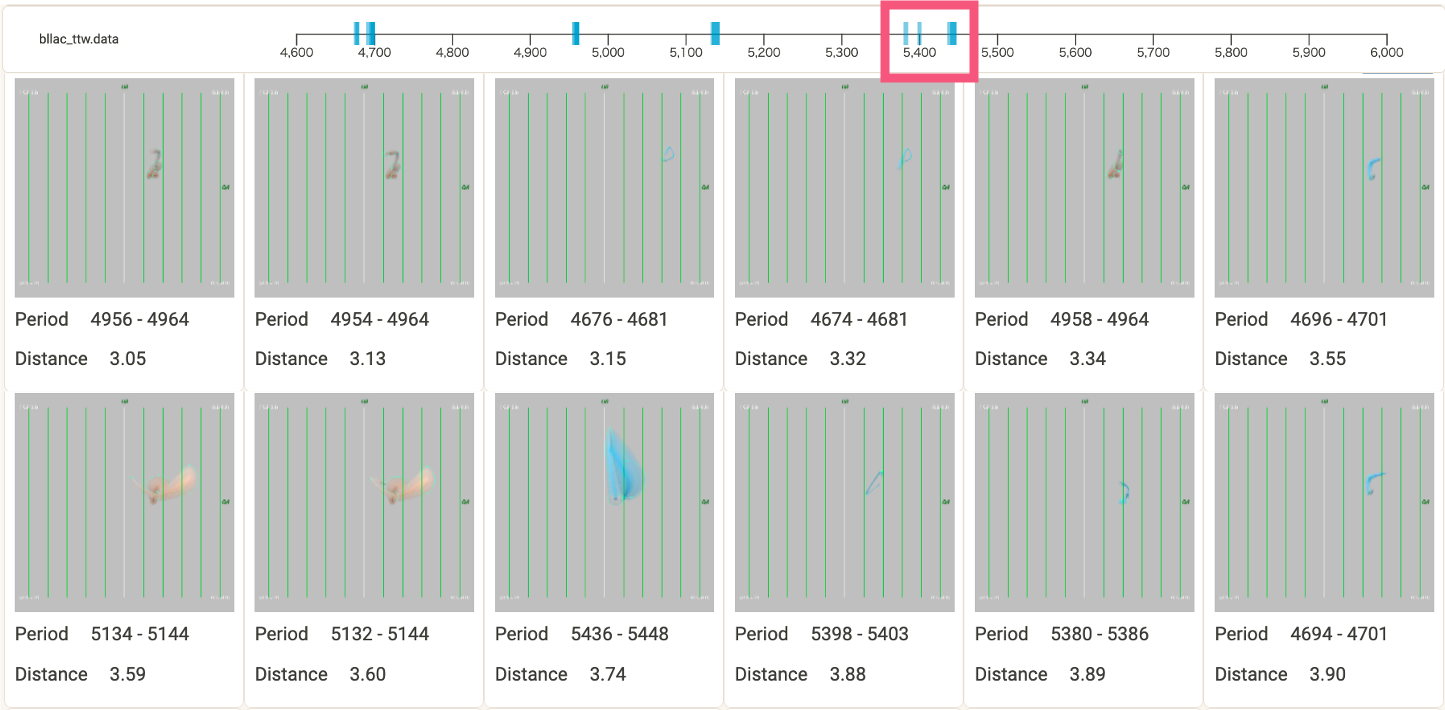
\includegraphics[width=.99\linewidth]{figures/correlateResultsLabel14.png}\\
    \footnotesize{\sf(c)~The top twelve time intervals that are similar to the query in (a).}\\
    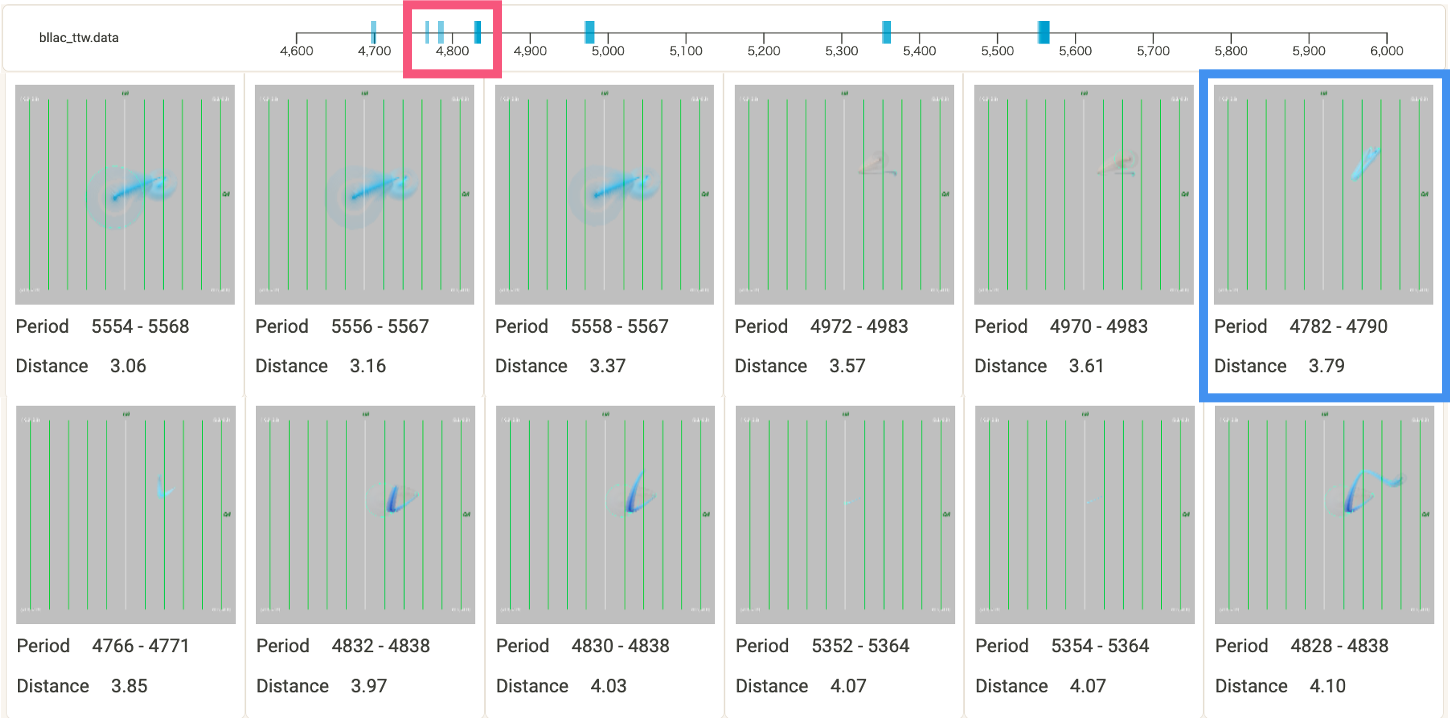
\includegraphics[width=.99\linewidth]{figures/anticorrelateResultsLabel14.png}\\
    \footnotesize{\sf(d)~The top twelve time intervals that are similar to the query in (b).}
    \caption{Analysis of the blazar \emph{BL Lac} to investigate correlation patterns between $I$ and $PD$. (a) and (b) are user-drawn sketches. (c) and (d) are the results of QBS with the queries shown in (a) and (b), respectively.}
    \label{fig:EvaluationQueryResults}
\end{figure}
%
Astronomer 1's goal in these case studies was to identify global statistical features of the period of interest and to build a hypothesis of correlations between the time variations of $I$ and $PD$.
To achieve this goal, he had to meticulously analyze correlations between $I$ and $PD$ in the entire time period and many short time intervals within that period.
However, it seemed difficult to manually examine each of the short time intervals.
Therefore, he decided to utilize QBS to investigate correlation patterns in a long-term observation dataset.

First, he formulated a hypothesis that an increase in $I$ tends to correlate with an increase in $PD$ in \emph{BL Lac}.
To validate this hypothesis and examine how frequently such behavior appears, he sketched the query shown in Fig.~\ref{fig:EvaluationQueryResults}~(a), 
where the $x$ and $y$ axes express $q$ and $u$, respectively, 
and the stroke width represents $I$.
Therefore, the input sketch indicates a pattern 
that $I$ gradually increases and then decreases in a way that is correlated to $PD$.
To extract time intervals with a similar shape but different position or different scale, he used the normalization and polar coordinates options. 
To avoid missing short events, he set the warping window size and the sliding window size to 0 and 2, respectively.

Fig.~\ref{fig:EvaluationQueryResults}~(c) shows the top twelve results of the query sketched in (a).
The timeline at the top of (c) illustrates 
that the extracted time intervals seem to be distributed over the entire dataset.
However, in the period from $[5{,}350, 5{,}450]$ (enclosed by a red rectangle in (c)), 
the input pattern seems to occur more frequently than in other periods.
Visiting all time intervals in this period individually and analyzing them in the TimeTubes view,
some of them include the correlation pattern in (a),
but others do not.
Thus, he concluded that the input correlation pattern does not frequently occur in that period.
The reason for this misclassification could be that our system, when using the normalization option, detects time intervals with a relatively small variation of $I$ as well.
However, he was still highly pleased with TimeTubesX, as it allowed him to quickly identify a relatively small number of time intervals that he could then examine in more detail.

\subsection{Case Study 2: Anticorrelation Patterns of $I$ and $PD$}\label{sec:anticorrelate}
Astronomer 1 also noticed that the variation in $I$ tends to anticorrelate with that in $PD$.
To detect time intervals with such anticorrelated $I$ and $PD$ patterns, he drew another query (Fig.~\ref{fig:EvaluationQueryResults}~(b))
where the plane represents the Stokes plane and the stroke width $I$.
The sketch describes a pattern in which $I$ gradually increases and then decreases, while $PD$ shows a negative correlation with $I$. 
He used the same parameters as in Section~\ref{sec:correlate}.

Fig.~\ref{fig:EvaluationQueryResults}~(d) shows the top twelve results of the query shown in (b).
Like in the previous case study, 
extracted time intervals seem to be distributed over the entire dataset.
However, in the period from $[4{,}750, 4{,}850]$ (enclosed by a red rectangle in (d)), 
the input pattern seems to occur more frequently.
Astronomer~1's group previously reported that, statistically, the variation in $I$ anticorrelates with that in $PD$ from the years 2008 to 2010 in \emph{BL Lac}~\cite{Gaur2014}.
However, even in that previous report, they did not analyze short time intervals in the period individually.
By analyzing the extracted time intervals in the period with TimeTubesX, he could verify not only that an increase in $I$ globally tends to co-occur with a decrease in $PD$, 
but also that local peaks of $I$ are correlated with decreases in $PD$.

These case studies with QBS underline the importance of local analysis of short time intervals within a larger time period in addition to a global analysis of the entire period.

\subsection{What-If Scenario Analysis}\label{sec:whatif}
This section explains how astronomers can identify what generally contributes to the $PD$ variation in blazars in a certain time period. 

Astronomers expect that $PD$ variation in a blazar is due to one of the two following hypotheses:
\begin{enumerate}[nosep, label=\textsl{Hypothesis \arabic*}:, ref=\textsl{Hypothesis \arabic*}, align=parleft, leftmargin=*]
    \item \textsl{$total\,flux$ increases (decreases) due to the increase (decrease) in $unpolarized\,flux$};  \label{scenario1}
    \item \textsl{There are two polarized components, and they are perpendicular to each other}. \label{scenario2}
\end{enumerate}
Note that $PD$ can be derived from the amount of $flux$: $PD = \frac{polarized\,flux}{total\,flux}$,
where $total flux = I = polarized\,flux + unpolarized\,flux$.
Astronomers can identify which of the above hypotheses contributes to the decrease in $PD$
by comparing time variations of data samples at the time intervals in the $q - u$ domain and in the $Q-U$ domain,
where $q = Q / I$ and $u = U / I$, as explained in Section~\ref{sec:BlazarData}.
In the case of \ref{scenario1}, the position of a data sample in the $q - u$ domain gradually moves toward the origin ($(q, u) = (0, 0)$),
whereas the position in the $Q-U$ domain does not move toward the origin ($(Q, U) = (0, 0)$)
because only the amount of $total flux$ increases.
On the other hand, in the case of \ref{scenario2}, 
$PD$ decreases due to a flare of another polarized component with $PA$ being perpendicular to the jet direction.
The position of a data sample moves toward the origin both in the $q - u$ domain and in the $Q - U$ domain 
because another polarized component influences the observed $Q$ and $U$ values, 
meaning that $q$ and $u$ (fractional values of $Q$ and $U$) are also influenced.
By comparing the datasets for $(q, u)$ and $(Q, U)$ with the side-by-side option in the visual data fusion~\cite{Fujishiro2018},
the plausibility of these hypotheses can be visually determined.
\begin{figure}[tb]
    \centering
    \includegraphics[width=.8\linewidth]{figures/stokesComparisonLabel.png}
    \caption{Comparison of a dataset consisting of $q$ and $u$ (left) and one consisting of $Q$ and $U$ (right) for the time interval $[4{,}782, 4{,}890]$.
    In both images, the position of the data sample goes toward the origin of the domain (lower left), which means that this polarization variation was caused by a decrease in the $PD$ of a different polarized component.}
    \label{fig:comparisonQIUIvsQU}
\end{figure}

The following discussion considers the anticorrelation patterns of $I$ and $PD$, as mentioned in Section~\ref{sec:anticorrelate}.
Astronomer 1 compared a dataset consisting of $q$ and $u$ with one consisting of $Q$ and $U$. The comparison results at the time interval with a blue rectangle displayed in Fig.~\ref{fig:EvaluationQueryResults}~(d) are shown in Fig.~\ref{fig:comparisonQIUIvsQU}.
As the red arrows in Fig.~\ref{fig:comparisonQIUIvsQU} indicate, 
he found that both data samples move toward the origin.
He found similar behavior at all short time intervals in the period $[4{,}750, 4{,}850]$.
Thus, he finally concluded that the negative correlation of $I$ and $PD$ in the period is not due to the increase in $unpolarized flux$ (\ref{scenario1}) but is instead due to the presence of two polarized components (\ref{scenario2}). 

Overall, TimeTubesX greatly facilitated this detailed visual exploration of blazar data. This allowed Astronomer 1 to examine many small time intervals with specific features, which would have been too laborious with previous methods.

\subsection{Qualitative Feedback from Domain Experts}\label{sec:feedback}
Astronomer 2 found that the rotation detection was useful. 
With TimeTubesX's rotation detection functionality, 
he was able to find three unknown rotation behaviors with a shifted rotation center in the blazar \emph{3C 454.3}~\cite{Huang2019}. 
Astronomers 1, 3, and 4 mentioned that the QBS method was especially useful and helpful for validating their high-level hypotheses, as demonstrated in Sections~\ref{sec:correlate} and \ref{sec:anticorrelate}. 
In particular, Astronomers 3 and 4 said that dynamic visual querying could be a powerful tool to examine jet physical processes and behaviors of plasma and magnetic fields under extreme conditions because the method can efficiently address arbitrary variation patterns of polarization, intensity, and color over time. Astronomers 1 and 3 noticed TimeTubesX’s potential for data mining. In particular, Astronomer 3 saw massive potential for mining existing and upcoming large polarization surveys, while Astronomer 1 found that using TimeTubesX will enable astronomers to identify interesting features in short time intervals to an extent that cannot be achieved with conventional methods due to too many short time intervals in a long-term dataset. Furthermore, fact-guided querying was impressive to him because it allows astronomers to refine their sketches based on actual extracted patterns.
